\documentclass{article}
\title{\Huge Aircraft Structures - I}
\Large{\author{$\mathcal{WAFFLE'S\ \ CRAZY\ \ PEANUT}$}}
\date{(Last updated: 28/4/14)}
\usepackage{enumerate}
\usepackage{amssymb}
\usepackage{caption}
\usepackage{tikz-qtree}
\usetikzlibrary{trees}
\usepackage{graphicx}
\usepackage{caption,subcaption}
\usepackage{calc}
\usepackage{amsmath}
\usepackage{import}
\newcommand{\para}[1]{\paragraph{#1}\mbox{}\\}
\usepackage{pgf,tikz}
\usetikzlibrary{arrows}
\usetikzlibrary{decorations.markings}
\pagestyle{empty}
\pagenumbering{gobble}
\newcommand{\degre}{\ensuremath{^\circ}}
\newcommand{\twoheaduparrow}{\mathrel{\rotatebox{90}{$\twoheadrightarrow$}}}
\begin{document}
\maketitle
\textbf{\section{\huge Static Determinacy of Structures}}
\
{\Large 
\para{\LARGE Mechanics Recall:}
\newline
\textbf{Coplanar forces} - confined to a common plane, can be parallel or concurrent. Their general resolution is,
{\LARGE $$\sum F_x=0,\ \sum F_y=0,\ \sum M_P=0$$}
\\
Sum of forces along the ``mutually perpendicular" directions is zero, and the sum of moments (including those contributed by the forces) about any point is \textbf{zero}.
\begin{enumerate}[(i)]
\item For \textit{concurrent forces}, the equilibrium conditions $\sum F_x=0$ and $\sum F_y=0$ are enough.
\item For \textit{parallel forces} the conditions $\sum F=0$ along direction of the forces, and $\sum M_P=0$ are suffice to resolve them.
\end{enumerate}
\newpage
\subsection{\LARGE Plane Truss Analysis}
$\ $
\paragraph{\Large Static Indeterminacy:}
\begin{itemize}
\item If the number of unknown reactions developed $>$ number of static equilibrium equations, then it is a  \textbf{statically indeterminate} structure.

(While trusses can make such cases statically determinate ``externally", they themselves need to be statically determinate ``internally").
\item The stability of a truss work is governed by
{\LARGE $$n=2j-3$$} $n=$ number of members, $\ j=$ number of joints
\begin{enumerate}[(a)]
\item $\mathrm{LHS=RHS}$: Structure is statically determinate, and it's a safe-life design (i.e) the structure can survive for a long time.
\item $\mathrm{LHS>RHS}$: Structure is statically indeterminate ``internally", and it corresponds to a fail-safe design (i.e.) the structure can survive on the event of failure (even if one member fails, other members can still be able to hold the structure).
\item $\mathrm{LHS<RHS}$: It's no longer a structure. It's a mechanism, which collapses as a whole.
\end{enumerate}
\end{itemize}
\newpage
\paragraph{\Large Assumptions made:}
\begin{itemize}
\item Members are pin-joined.
\item Members resist the point loads in the form of tension and compression.
\item Loads are applied only at joints.
\end{itemize}
\begin{figure}
\caption*{\Large \textbf{Figure 1: Plane Truss (Example)}}
\hbox{\hspace{-4.5cm}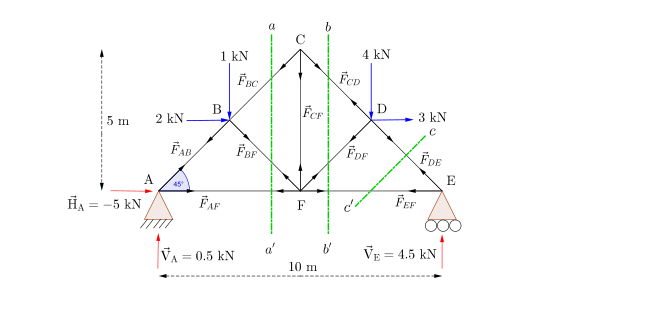
\includegraphics[scale=1.35]{Truss.pdf}}
\end{figure}
\newpage
\paragraph{\Large Methods:}
\begin{enumerate}[(i)]
\item Method of Joints
\item Method of Section
\item Method of Shear
\end{enumerate}
\subsection{\LARGE Method of Joints}
Resolve the forces joint by joint.
\paragraph{\Large Procedure:}
\begin{enumerate}[(a)]
\item Find the reaction at the supports, and check whether the truss work is statically determinate externally and internally.
\item Choose a ``resolvable" joint* (where the number of unknown reactions $\leq$ the number of equilibrium equations) and find the tension on the members.
\item As the forces are concurrent, the equilibrium equations $F_x=0$ and $F_y=0$ are suffice to resolve.
\newline

*\textbf{Note:} Some joints may have a greater number of unknowns. For e.g., joint $\mathrm F$ in the above truss has five tensile forces acting on it. They can be used to check the calculations.
\end{enumerate}
\newpage
\paragraph{\Large Keep in mind:}
\begin{enumerate}[1)]
\item Forces are \textit{assumed} to be tensile at all joints (i.e) they act away from the joints.
\item The mutually perpendicular directions can be in any orientation. Even a tangent and normal to a given joint can do the resolution of forces.
\item Don't confuse yourselves with \textbf{Newton's third law}. This convention does not mean that.

For e.g., in the above truss, $F_{AB}$ is the tension between $\mathrm A$ and $\mathrm B$. At joint $\mathrm A$, $\vec F_{AB}$ acts from $\mathrm A\to\mathrm B$, whereas at the joint $\mathrm B$, it acts from $\mathrm B\to\mathrm A$, according to our assumption (see \textbf{1st}).

But, it's true. Because, tension is similar to reaction. You resolve it once, and get the direction, then that direction remains the same throughout the problem. So, $\vec F_{AB}=\vec F_{BA}$
\end{enumerate}
\subsection{\LARGE Method of Section:}
Slice the given structure into sections. As the truss needs tensile and compressive forces to be stable, you apply the tensile forces manually at the loose ends of the section, and resolve them.
\newpage
$\ $
(It's very similar to D'Alembert's principle, used to analyze an accelerating object, wherein you provide an opposing force to balance the acceleration of the object, and thereby resolve it using static equilibrium eqns.)
\\
\\
Slicing is shown in Fig.1 by $aa'$, $bb'$ and $cc'$.

\paragraph{\Large Procedure:}
\begin{enumerate}[(a)]
\item Slice the structure appropriately between joints. No more than 3 unknown forces should appear, for the sliced part to be statically determinate ``internally".
\item Use the moment equilibrium condition (i.e.) moment about any point, $\vec M_P=0$.
\newline

\textbf{\Large Keep in mind:} Moment is simply force times the ``perpendicular distance" $(\vec M=\vec r\times \vec F)$. So, the forces that pass through the point do not contribute any moment. And, while resolving, stick to a particular direction (clockwise/anticlockwise).
\\

For example, taking left slice of $aa'$ in Fig.1, moments $\vec M_A$, $\vec M_F$ and $\vec M_B$ can be equated to zero.
\\
\\
Regarding the perpendicular distance, (for e.g.) while using $\vec M_F=0$, $\mathrm{1\ kN}$ is at $r=\mathrm{2.5\ m}$ (horizontal), whereas $\mathrm{2\ kN}$ is at $r=\mathrm{2.5\ m}$ (vertical).
\end{enumerate}
\newpage
\subsection{\LARGE Space Truss}
Analyze the forces on members from the orthographically projected truss work.
\para{\Large Moment recall:}
$\ $
Moment is always taken about a line. So, the moment of a force about a line parallel to its direction is \textbf{zero!}
$$\mathrm{Moment=Force\times Perpendicular\ distance}$$
Moment is a vector. Its direction is perpendicular to the plane containing $\vec r$ and $\vec F$
{\LARGE $$\vec M=\vec r \times \vec F$$}
Resolution of moments, and magnitude of net moment are similar to that of the forces,
{\LARGE $$M=\sqrt{{M_x}^2+{M_y}^2+{M_z}^2}$$}
\paragraph{\Large Note:}
\begin{itemize}
\item When a force is transferred from one point to another point, it goes as a force with same magnitude and direction, but also with a moment.
\item Just as forces are indicated by arrows ($\rightarrow $), moments are indicated by double-headed arrows ({\huge $\twoheadrightarrow $}). Their rotation is given by one of the thumb rules, left/right depends on the question.
\end{itemize}
\newpage
\paragraph{\Large Procedure:}
\begin{enumerate}[(a)]
\item If the given members are in 3D space, then project them orthographically in 2D (front and side views).
\item Tabulate the distances of members relative to the vertical or horizontal (for each $D$, $S$, and $V$).
\item Find the magnitude of the net distance using,
{\LARGE $$|L|=\sqrt{D^2+S^2+V^2}$$}
\item Find {\LARGE $D\over L$},{\LARGE $S\over L$}, and {\LARGE $V\over L$}.
\item Now that the direction cosines are found, apply the force equilibrium to find the forces on members,
\begin{center}
{\LARGE $\sum F_i\cdot \frac{D}L=0$}, {\LARGE $\sum F_i\cdot \frac{S}L=0$}, {\LARGE $\sum F_i\cdot \frac{V}L=0$}
\end{center}
\end{enumerate}
$\ $
\\
\textbf{\Large Note:} 
\begin{itemize}
\item All the forces should be accounted for equilibrium (including the externally applied ones, with appropriate SI units).
\item $D$, $S$ and $V$ \textit{can} be negative, when the members extend from the origin to the negative region of the co-ordinate system
\end{itemize}
\newpage
{\LARGE For a point load $P$ at a distance $a$ from support,}
\begin{figure}
\caption*{\Large \textbf{Figure 2: Simply-supported Beam}}
\hbox{\hspace{-2.2cm}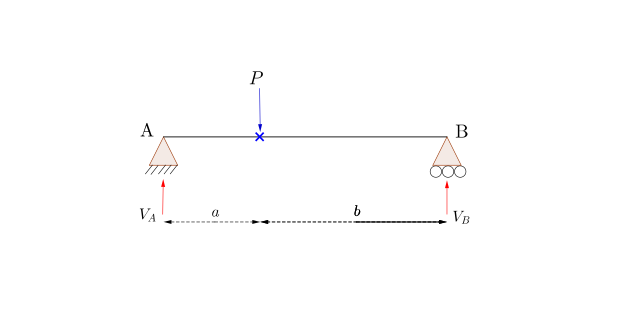
\includegraphics{Beam_A.pdf}}
\end{figure}
\begin{enumerate}[(i)]
\item Maximum Bending Moment: {\LARGE $$M_{max}=\frac{Pab}{l}$$}
\item Maximum deflection:
{\LARGE $$\delta_{max}=-\frac{Pa^2b^2}{3EIl}{}$$}
\end{enumerate}
\newpage
{\LARGE For a distributed load of intensity $q$,}
\begin{figure}
\caption*{\Large \textbf{Figure 3: Simply-supported Beam}}
\hbox{\hspace{-2.2cm}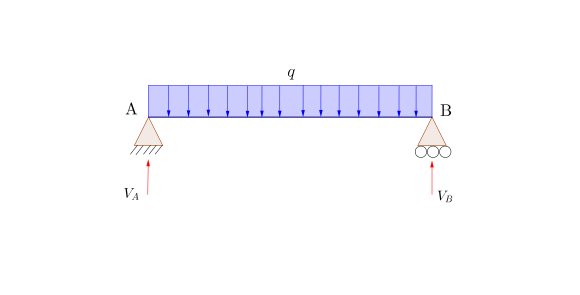
\includegraphics{Beam_B.pdf}}
\end{figure}
\begin{enumerate}[(i)]
\item Maximum Bending Moment: {\LARGE $$M_{max}=\frac{ql^2}{8}$$}
\item Maximum deflection:
{\LARGE $$\delta_{max}=-\frac{5ql^4}{384EI}{}$$}
\end{enumerate}
-\newpage
{\LARGE For point load $P$ at a distance $a$ from fixed end,}
\begin{figure}
\caption*{\Large \textbf{Figure 3: Cantilever Beam}}
\hbox{\hspace{-2.2cm}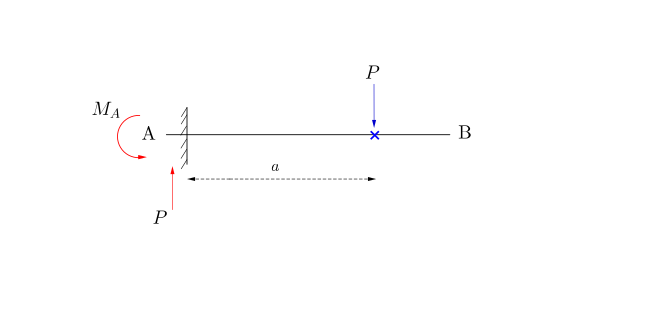
\includegraphics{Beam_C.pdf}}
\end{figure}
\begin{enumerate}[(i)]
\item Maximum Bending Moment: {\LARGE $$M_{max}=-Pa$$}
\item Slope at B: {\LARGE $$\theta_B=-\frac{Pa^2}{2EI}$$}
\item Maximum deflection:
{\LARGE $$\delta_{max}=-\frac{Pl^2}{6EI}\ (3l-a)$$}
\end{enumerate}
\newpage
\subsection{\LARGE Clapeyron's 3-moment equation:}
\paragraph{\Large Procedure:}
\begin{enumerate}[(a)]
\item Split the given indeterminate beam into spans, and use Clapeyron's equation for the spans. Each span should be ``statically determinate".
{\LARGE $$M_1L_1\ +\ 2M_2(L_1+L_2)\ +\ M_3L_2=\ -\ \frac{6A_1a_1}{L_1}\ -\ \frac{6A_2b_2}{L_2}$$}
\\
{\LARGE $L_1$, $L_2$} = Lengths of spans considered

{\LARGE $M_1$, $M_2$, $M_3$} = Support moments

{\LARGE $A_1$, $A_2$} = Area of Bending moment diagrams

{\LARGE $a_1$, $b_2$} = Centroidal distance from moment diagrams
\\
\item Apply the formula for two spans at a time, to obtain a solvable set of equations.
\item Solve the equations to get the moments.
\item Take moments at the right/left of a support from a certain joint, to get the respective reactions.
\end{enumerate}
\subsection{\LARGE Moment Distribution method:}
\begin{itemize}
\item {\LARGE $\mathrm{Stiffness\ factor:}$} Factor (a number) multiplied to the magnitude of couple required to produce unit rotation at that end of span.
{\LARGE $$\bigg(\frac{4EI}{L},\ \frac{3EI}{L}\bigg)$$}
\paragraph{\Large Note:} If one end of the chosen span has a moment, then the other end has a stiffness factor of $4$. If not, then it becomes $3$.
\item {\LARGE $\mathrm{Distribution\ factor:}$} Fraction of chosen stiffness factor with respect to the total stiffness factor at the chosen joint.
{\Large $$\bigg(\frac{sf_1}{sf_1+sf_2},\ \frac{sf_2}{sf_1+sf_2}\bigg)$$}
\item {\LARGE $\mathrm{Carry-over\ factor:}$} When an external moment is applied, {\LARGE $50$} \% of the moment is carried over to near end of the span, \textbf{provided} the joint has a moment.
\item {\LARGE $\mathrm{Fixed-end\ moments:}$} Moments in the member when it's fixed against rotation.
{\LARGE $$\bigg(\frac{Pa^2b}{L^2},\ \frac{Pab^2}{L^2},\ \frac{qL^2}{12}\bigg)$$}
\end{itemize}
\paragraph{\Large Procedure:}
\begin{enumerate}[(a)]
\item Write the factors, and calculate fixed-end moments.
\item Apply counter moments at the extreme ends of beam, which is then carried over to near end of the span.
\item Any unbalanced moment at a particular joint is now shared on either side as per the distribution factor. (carry-over if any, is also taken into account)
\item Sum up the values of moments and iterate (c) till there's a repetition in the moment values.
\end{enumerate}
\begin{figure}
\hbox{\hspace{-9.2cm}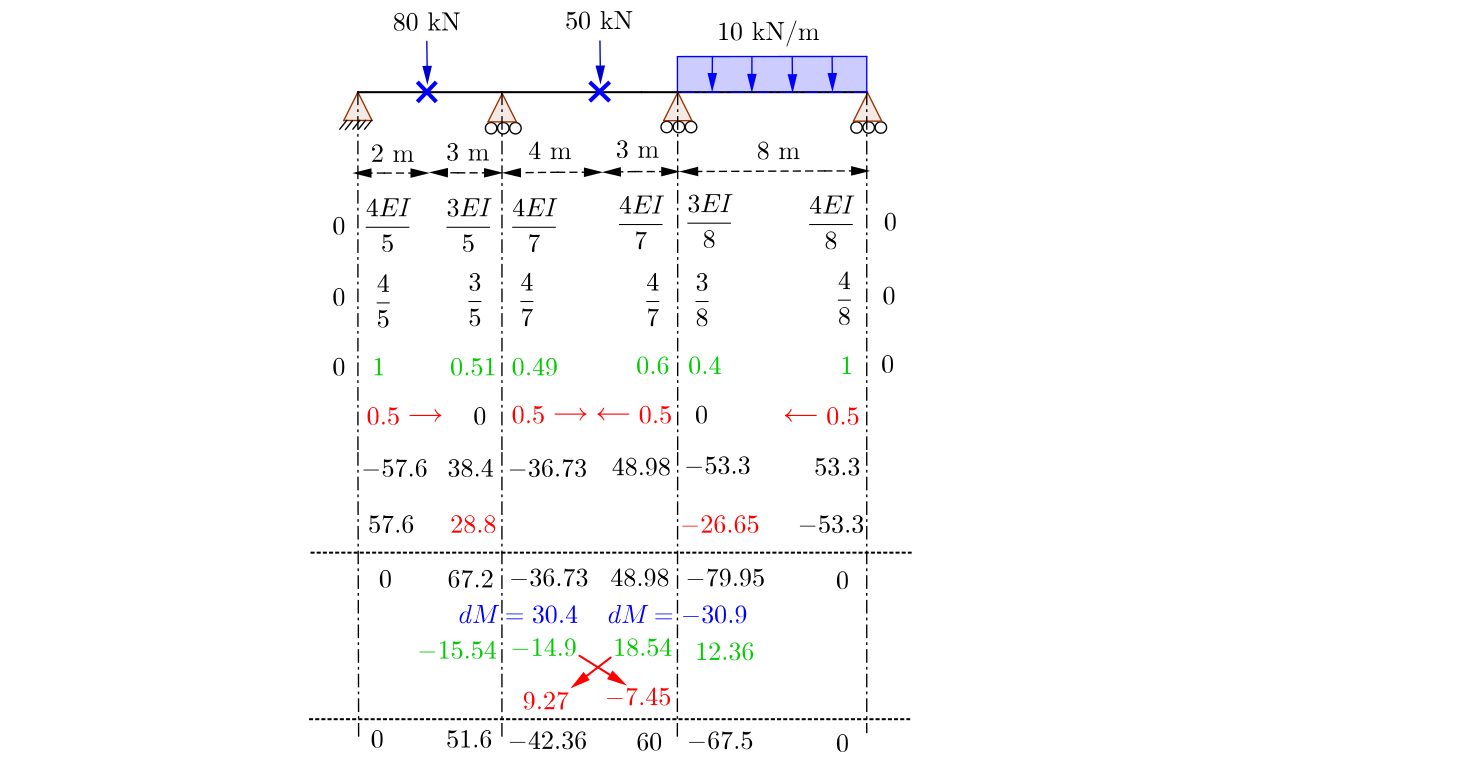
\includegraphics[scale=0.9]{Moment.pdf}}
\caption*{\Large \textbf{Figure 2: Moment-Distribution (Example)}}
\end{figure}
\newpage
\textbf{\section{\huge Failure Theories}}
\subsection{\LARGE Maximum Principal Stress Theory:}
$\ $
{\LARGE $$\tau_{\mathrm{max}}=\frac{T r_{\mathrm{max}}}{J}$$
$$\sigma_{\mathrm{max}}=\frac{M_{\mathrm{max}}\ y}{I}$$
\newline
Principal stresses,
$$\sigma_{1,2}=\frac{\sigma_{xx}+\sigma_{yy}}{2}\pm\sqrt{\bigg(\frac{\sigma_{xx}-\sigma_{yy}}{2}\bigg)^2+\tau_{xy}^2}$$
$\ $
$$\mathrm{Max}\ (\sigma_1,\sigma_2)<\sigma_{yp}$$}
\paragraph{\Large Theory of Rankine \& Mohr: (Procedure)}
\begin{enumerate}[(i)]
\item Positive axes correspond to tensile {\LARGE $\sigma_{yp}$}, whereas negative axes correspond to compressive {\LARGE $\sigma_{yp}$}. Form a rectangle from the values.
\item For Rankine, check whether {\LARGE $\mathrm{Max}\ (\sigma_1,\sigma_2)$} lies within the rectangle.
\item For Mohr, join {\LARGE $\sigma_t$} and {\LARGE $\sigma_c$}  to form a trapezium and finally check the same.
\end{enumerate}
\subsection{\LARGE Maximum Principal Strain Theory:}
$\ $
{\LARGE $$\epsilon_1=\frac{1}E\ \big(\sigma_1-\nu(\sigma_2+\sigma_3)\big)$$
\begin{flushright}
$\forall\ \sigma_1>\sigma_2>\sigma_3$
\end{flushright}
Condition for safety,
$$\sigma_1-\nu(\sigma_2+\sigma_3)<\sigma_{yp}$$}
For a \textbf{thin-walled cylinder}, $$\bigg(\frac{r}t>10\ \ \mathrm{and}\ \ \frac{d}t>20\bigg)$$
{\LARGE $$\sigma_c=\frac{pr}t\ \ \sigma_t=\frac{pr}{2t}$$
$\ $
$$\sigma_c<\sigma_{yp}$$}
\subsection{\LARGE Maximum Shear Stress Theory:}
$\ $
{\LARGE $$\tau_{\mathrm{max}_1}=\frac{\sigma_1-\sigma_2}{2}, \ \ \tau_{\mathrm{max}_2}=\frac{\sigma_2-\sigma_3}{2},\ \ \tau_{\mathrm{max}_3}=\frac{\sigma_3-\sigma_1}{2}$$}
{\LARGE $$\mathrm{Max}\ \big(|\tau_1|,|\tau_2|,|\tau_3|\big)<\frac{\sigma_{yp}}2$$}
\subsection{\LARGE Octahedral Shear Stress Theory:}
{\LARGE $$(\sigma_1-\sigma_2)^2+(\sigma_2-\sigma_3)^2+(\sigma_3-\sigma_1)^2<2\sigma_{yp}^2$$}
\subsection{\LARGE Maximum Strain Energy Theory:}
{\LARGE $$\sigma_1^2+\sigma_2^2+\sigma_3^2-2\nu(\sigma_1\sigma_2+\sigma_2\sigma_3+\sigma_3\sigma_1)<\sigma_{yp}^2$$}
\end{document}